\chapter{Wprowadzenie}
Jendym z zastosowań teleinformatyki w dzisiejszych czasach jest monitorowanie i automatyzacja procesów zachodzących w budynkach mieszkalnych i biurowych. 
W większości nowoczesnych budynków biurowych zamontowane są liczne urządzenia zapewniające komfortowe warunki pracy osób przebywających w biurach takie jak np. klimatyzatory czy nawilżacze powietrza. Te jak i inne urządzenia HVAC (Heating, Ventilation, Air Conditioning czyli ogrzewanie, wentylacja i klimatyzacja) mają moc liczoną w kilowatach.

Opłata za energię elektryczną potrzebną do funkcjonowania sieci takich urządzeń, jest częścią kosztu mediów (prądu, wody, ogrzewania, odprowadzania ścieków), które średnio stanowią ponad jedną trzecią miesięcznych kosztów utrzymania budynku \cite{bib:raportKoszty}.

Założeniem systemu tworzonego na potrzeby tej pracy jest obniżenie kosztów związanych z działaniem klimatyzacji z zachowaniem komfortu użytkowników budynku. 
System będzie miał do dyspozycji informacje zbierane z sensorów (małych czujników odczytujących wartości różnych parametrów) rozmieszczonych w każdym biurze oraz dane o wykorzystaniu pomieszczeń. \seefigure{generalContextDiagram}

\begin{figure}[bth]
    \centering
    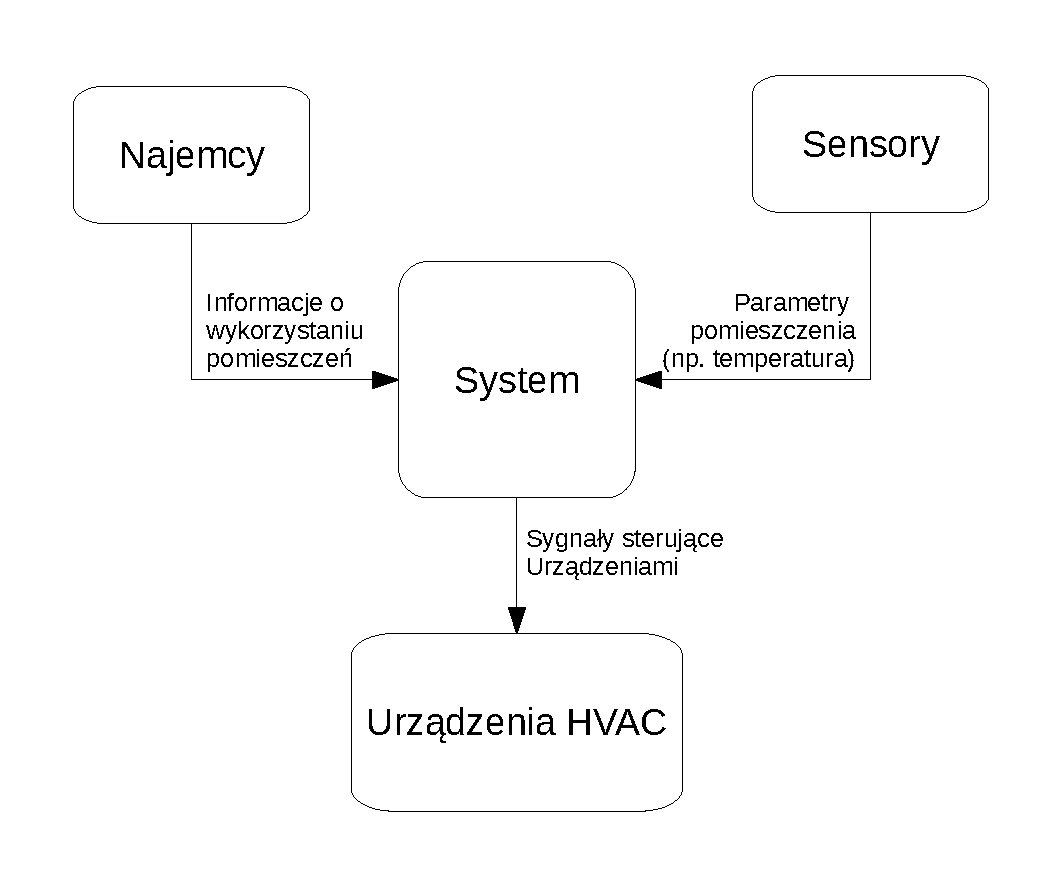
\includegraphics[width=0.7\textwidth]{./diagrams/GeneralContextDiagram.pdf}
    \caption{Kontekst systemu}
    \label{fig:generalContextDiagram}    
\end{figure}
 

Kalendarze firmowe są głównym źródłem informacji, w których pomieszczeniach i w jakich godzinach, odbywają się spotkania. Można wyobrazić sobie inne źródła, jak np. lokalizacja pracowników przypisanych do pomieszczenia. 
Jednak implementowany system będzie skupiał się głównie na wydarzeniach firmowych, jako że są mniej dynamiczne i można za ich pomocą zamodelować również np. spóźniającego się pracownika przesuwając godzinę spotkania.

System będzie sterował urządzeniami HVAC poprzez aktuatory (urządenia pozwalające komputerowi wpływać na stan świata rzeczywistego), które mogłyby składać się z mikrokomputerów z portami podczerwieni lub komunikacją radiową (Bluetooth czy WiFi.)
Aktuatory wyręczałyby użytkowników w prawidłowym ustawianiu urządzeń.
Przy ręcznym ustawianiu komfortowej temperatury przez człowieka zwykle odbywa się to na początku spotkania, gdy uczestnicy uznają, że warunki w pomieszczeniu nie odpowiadają ich wymaganiom. 
Aby jak najszybciej pozbyć się tego uczucia, włączają najmocniejszy, lecz nie koniecznie najbardziej oszczędny, tryb w klimatyzatorach.

Oszczędność z zastosowania systemu będzie przychodzić z uruchomienia klimatyzatorów przed spotkaniem w najbardziej ekonomicznym wariancie tak, aby uczestnicy mieli komfortowe warunki od początku aż do końca spotkania. 

Do wyliczenia, ile czasu wcześniej należy uruchomić urządzenia, potrzebne są matematyczne modele zjawisk, takich jak wymiana ciepła. 
Tworzeniem precyzyjnych modeli takich zajwisk zajmują się inne dziedziny techniki - ogrzewnictwo oraz chłodnictwo. 
Jako, że opracowanie dokładnych modeli jest poza zakresem tej pracy system będzie korzystał z modelu uproszczonego. 

\subsection*{Cel projektu}
Celem projektu jest zaprojektowanie systemu, który będzie poszukiwać i wdrażać najbardziej oszczędny tryb pracy urządzeń HVAC. Optymalizacja kosztów spowodowana działaniem systemu nie powinna mieć niekorzystnego wpływu na komfort użytkowników.